\chapter{Comportamiento longitudinal}
\label{ch:longitudinal-model}

El comportamiento longitudinal es un problema de regresión sobre cómo ha de comportarse la aceleración del \gls{dvu}\index{driver-vehicle unit} en función de la información existente alrededor. Los perfiles de aceleración para los conjuntos de entrenamiento y de test se ilustran en la Figura~\ref{fig:acceleration-profiles}.

\begin{figure}
	\centering
	\subfloat[Entrenamiento]{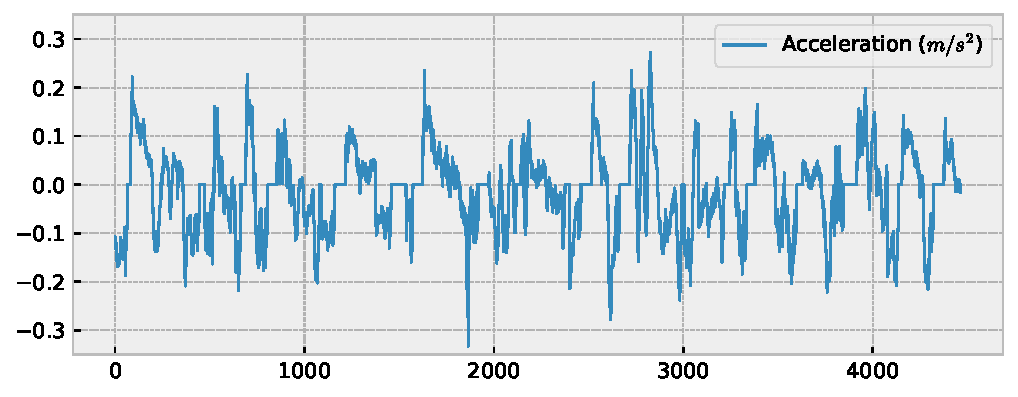
\includegraphics[width=\textwidth]{acceleration-profiles-training}}\qquad
	\subfloat[Test]{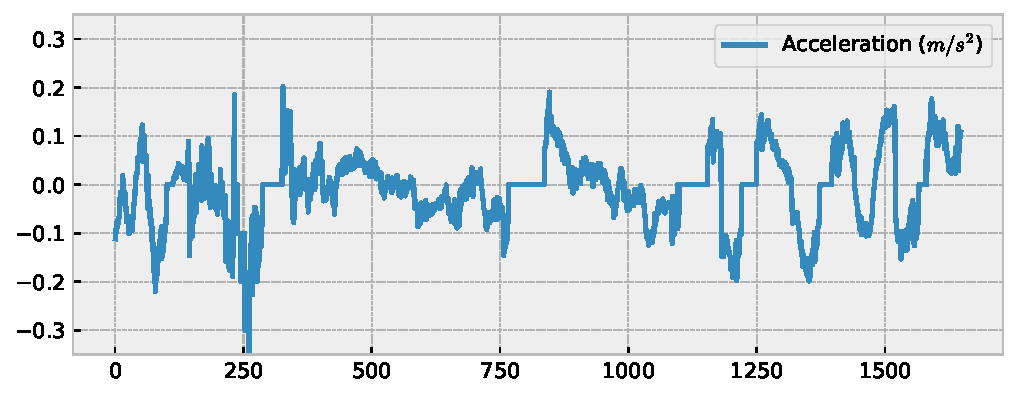
\includegraphics[width=\textwidth]{acceleration-profiles-test}}
	\caption[Perfiles de aceleración a ajustar por los modelos. Conjuntos de entrenamiento y de test]{Perfiles de aceleración durante los experimentos: (a) entrenamiento y (b) test. Estos son los conjuntos de datos que se intentarán ajustar con los modelos.}
	\label{fig:acceleration-profiles}
\end{figure}

Por la naturaleza del problema se han seleccionado dos técnicas diferentes para el ajuste del modelo:

\begin{enumerate}
	\item \Acrshort{mlp}\index{perceptron multicapa}. Al ser un problema de regresión, el uso de \acrlongplsp{mlp} en el comportamiento longitudinal está justificado al ser considerados éstos aproximadores universales\sidenote{
			El \textit{Teorema de aproximación Universal} \cite{hornik1991approximation} postula que un \acrlongsp{mlp}\index{perceptron multicapa} con al menos una capa oculta es capaz de aproximar cualquier función si dispone de suficientes neuronas en ésta.
	}.
	\item \Acrshort{fcs}\index{sistema de control borroso}. La formulación del problema se ajusta muy bien al funcionamiento de estos modelos. Además, los \acrlongplsp{fcs}\index{sistema de control borroso} tienen la ventaja de que se puede explicar su funcionamiento, a diferencia de los \acrlongplsp{mlp}\index{perceptron multicapa} con una o más capas ocultas.
\end{enumerate}

Ambos modelos se ajustarán con un procedimiento basado en el descenso del gradiente denominado ADAM~\cite{kingma2014adam}. Su aplicación a los \acrlongplsp{mlp}\index{perceptron multicapa} es directa (después de todo es una técnica desarrollada dentro de área de las \acrlongplsp{ann}\index{red neuronal artificial}), pero para los \acrlongplsp{fcs}\index{sistema de control borroso} es necesaria una representación que permita el uso de este método para su optimización. Esta representación es una de las aportaciones de esta tesis y se se explica en la sección \nameref{ss:fuzzy-controller-adjustment} más adelante en este capítulo.

El error que se trata de minimizar es el cuadrado del \gls{rmse}\index{RMSE} entre los valores de aceleración del conjunto real y los ajustados por el modelo. Los resultados no obstante se presentan con el \gls{rmse}\index{RMSE} ya que éste es directamente interpretable en las medidas de la variable sobre la que se aplica (en nuestro caso, \SI{}{\metre\per\square\second}).

\section{Ajuste de controladores borrosos por descenso del gradiente}
\label{ss:fuzzy-controller-adjustment}

Como vimos en la sección \nameref{ss:fcs} del capítulo \nameref{ch:sota-ci}, un \acrlongsp{fcs}\index{sistema de control borroso} se compone de cuatro bloques diferenciados: la fuzzificación, el bloque de reglas, la inferencia y la defuzzificación. De estos bloques, el proceso manual de ajuste se resume siempre en dos pasos\sidenote{
	Por supuesto implica más ajustes como la elección de las funciones de fuzzificación, las $t$-normas y $t$-conormas, de la función de defuzzificación, pero estas operaciones no tienen tanto impacto en el desempeño del controlador como las particiones borrosas y las reglas.
}:

\begin{enumerate}
	\item Elección de las particiones borrosas de las variables lingüísticas.
	\item Definición de las reglas borrosas.
\end{enumerate}

Las soluciones de ajuste que existen en la literatura suelen funcionar ajustando automáticamente uno de los dos puntos, manteniendo fijo el otro (e.g. ajustar las particiones fijas las reglas). Nosotros representaremos el controlador como un grafo computacional de manera que sus gradientes sean sencillos de ajustar\sidenote{
	Como veremos más adelante, el tiempo de ajuste con esta representación es muy rápido, lo que abre la posibilidad de desarrollar un algoritmo que incluya este para el ajuste de los metaparámetros del controlador, como por ejemplo los tamaños de las particiones.
}.

Se han tomado una serie de decisiones de diseño para facilitar el desarrollo del controlador, aunque son fácilmente modificables. Éstas son:

\begin{itemize}
	\item Para cada partición borrosa se limitarán las funciones de pertenencia a: una línea descendente para caracterizar al primer conjunto borroso\index{conjunto borroso}, una línea ascendente para caracterizar el último y trapezoides para caracterizar al resto.
	\item Las $t$-norma y $t$-conorma serán el máximo y el mínimo respectivamente. La $t$-norma se usará como operador asociado al \texttt{AND} lógico y a la operación de implicación, mientras que la $t$-conorma se usará como operador asociado al \texttt{OR} lógico y a la acumulación.
	\item El controlador será de tipo \textit{Takagi-Sugeno} de orden $0$, y por tanto se representarán las funciones de salida como conjuntos borrosos\index{conjunto borroso} de tipo singletón. La función de defuzzificación será la la operación CoGS\sidenote{
		La operación CoGS (\textit{Center of Gravity for Singletons}) se define como:
		\begin{equation}
		CoGS = \sum_{i=1}^n w_i \cdot o_i
		\label{eq:cogs}
		\end{equation}
		Es decir, la suma ponderada de los valores de salida.
	}.
	\item El tamaño de las particiones borrosas no variará dinámicamente a lo largo del entrenamiento, siendo éste un meta-parámetro de configuración del controlador.
	\item El controlador tendrá una única variable de salida.
\end{itemize}

\subsection{Representación de un \acrlongsp{fcs} como grafo computacional}

Sea $\mathcal{V} = {V_1, V_2, \ldots, V_n}$ el conjunto ordenado de variables lingüísticas de nuestro controlador, y sea $O$ la variable lingüística de salida. Cada una de estas variables tendrá un número prefijado de conjuntos $\mathcal{N} = {N_{V_1}, N_{V_2}, \ldots, N_{V_n}}$ para las variables de entrada y $N_O$ para la variable de salida.

El controlador recibirá una matriz bidimensional de rango $(m, n)$ y devolverá un vector de rango $(m)$, siendo $m$ el número de ejemplos que queremos calcular a la vez.

Representaremos el \acrlongsp{fcs}\index{sistema de control borroso} como grafo computacional. De esta manera, podremos (i) aplicar la función de manera más eficiente y (ii) calcular fácilmente los gradientes de las funciones parciales para aplicar la técnica del descenso del gradiente propagando el error de la salida.

El proceso de desarrollo será el siguiente: primero, construiremos cada uno de los bloques fundamentales del \acrlongsp{fcs}\index{sistema de control borroso} como un grafos computacionales; después construiremos el controlador conectando entre sí estos grafos.

\paragraph{Bloque de fuzzificación}

El grafo computacional asociado a este bloque tomará una matriz bidimensional de rango $(m, n)$ (la matriz de entrada) que contendrá para cada ejemplo una lista de los valores que toma cada una de las variables de entrada. La salida de este grafo será una matriz bidimensional de rango $(m, \sum_{i=1}^n N_i)$, donde se almacenarán los grados de pertenencia de esos valores acada conjunto borroso\index{conjunto borroso} de la variable que les corresponda (Figura~\ref{fig:input-to-fuzzy-input}).

\begin{figure}
	\centering
	\small
	\begin{equation*}
	\left(\begin{array}{>{\columncolor{red!20}}c>{\columncolor{blue!20}}cc}
	x^1_{V_1} & x^1_{V_2} & \ldots \\
	x^2_{V_1} & x^2_{V_2} & \ldots \\
	x^3_{V_1} & x^3_{V_2} & \ldots \\
	x^4_{V_1} & x^4_{V_2} & \ldots \\
	\end{array}\right)
	\rightarrow
	\left(\begin{array}{>{\columncolor{red!20}}c>{\columncolor{red!20}}c>{\columncolor{blue!20}}c>{\columncolor{blue!20}}cc}
	\mu^1_{V_1}(x^1_{V_1}) & \mu^2_{V_1}(x^1_{V_1}) & \mu^1_{V_2}(x^1_{V_2}) & \mu^2_{V_2}(x^1_{V_2}) & \ldots \\
	\mu^1_{V_1}(x^2_{V_1}) & \mu^2_{V_1}(x^2_{V_1}) & \mu^1_{V_2}(x^2_{V_2}) & \mu^2_{V_2}(x^2_{V_2}) & \ldots \\
	\mu^1_{V_1}(x^3_{V_1}) & \mu^2_{V_1}(x^3_{V_1}) & \mu^1_{V_2}(x^3_{V_2}) & \mu^2_{V_2}(x^3_{V_2}) & \ldots \\
	\mu^1_{V_1}(x^4_{V_1}) & \mu^2_{V_1}(x^4_{V_1}) & \mu^1_{V_2}(x^4_{V_2}) & \mu^2_{V_2}(x^4_{V_2}) & \ldots \\
	\end{array}\right)
	\end{equation*}
	\caption[Ejemplo de operación en el bloque de fuzzificación]{El bloque de fuzzificación transformará los valores de sus respectivos dominios al de cada conjunto borroso. La matriz generada tendrá tantas columnas como conjuntos borrosos posee cada variable.}
	\label{fig:input-to-fuzzy-input}
\end{figure}

Para ello, se le aplicará a cada columna de la matriz de entrada tantas operaciones (funciones de pertenencia) como conjuntos borrosos\index{conjunto borroso} posea. Concretamente se aplicarán operaciones de línea descendente, trapezoidal y ascendente.

Los grafos de las líneas \textbf{ascendente} y \textbf{descendente} tienen una forma parecida. El grafo asociado a la fórmula de la línea descendente se muestra en la Figura~\ref{fig:slope-asc-grap}, que es la que se correspondería con el último conjunto de una partición borrosa. Como se puede ver, las variables ajustables son $a$ y $\delta b$. Estas definen el intervalo $(a, a + \delta b) \in \mathbb{R}$ donde los valores $f(X)$ ascienden de $0$ a $1$ (o descienden de $1$ a $0$ en el caso de la recta ascendente).

\begin{figure}
	\centering
	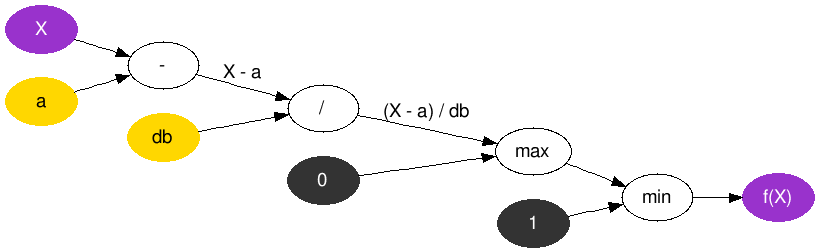
\includegraphics{slope-asc-graph}
	\caption[Grafo computacional de la función de pertenencia para la línea ascendente]{Ilustración del grafo computacional para la función de pertenencia línea ascendente. La fórmula que describe es $\mu(x) = \min(\max(\frac{x - a}{\delta b}, 0), 1)$, quedando acotada $\mu(x)$ en el intervalo $[0, 1] \in \mathbb{R}$. El grafo computacional para la línea descendente es similar y se corresponde con la fórmula $\mu(x) = \min(\max(\frac{a - x}{\delta b + 1}, 0), 1)$.}
	\label{fig:slope-asc-grap}
\end{figure}

El \textbf{trapecio} se define a partir de los parámetros $(a, \delta b, \delta c, \delta d) \in \mathbb{R}$, que definen los intervalos $I_1 = (a, a + \delta b)$, $I_1 = (a + \delta b, a + \delta b + \delta c)$ y $I_3 = (a + \delta b + \delta c, a + \delta b + \delta c + \delta d)$. $I_1$ es el intervalo donde la función de pertenencia aumenta su valor de $0$ a $1$, $I_2$ el intervalo superior del trapecio donde la función vale $1$ e $I_3$ donde la función comienza a descender su valor de $1$ a $0$. El grafo asociado a esta función se ilustra en la figura~\ref{fig:trap-graph}

\begin{figure}
	\centering
	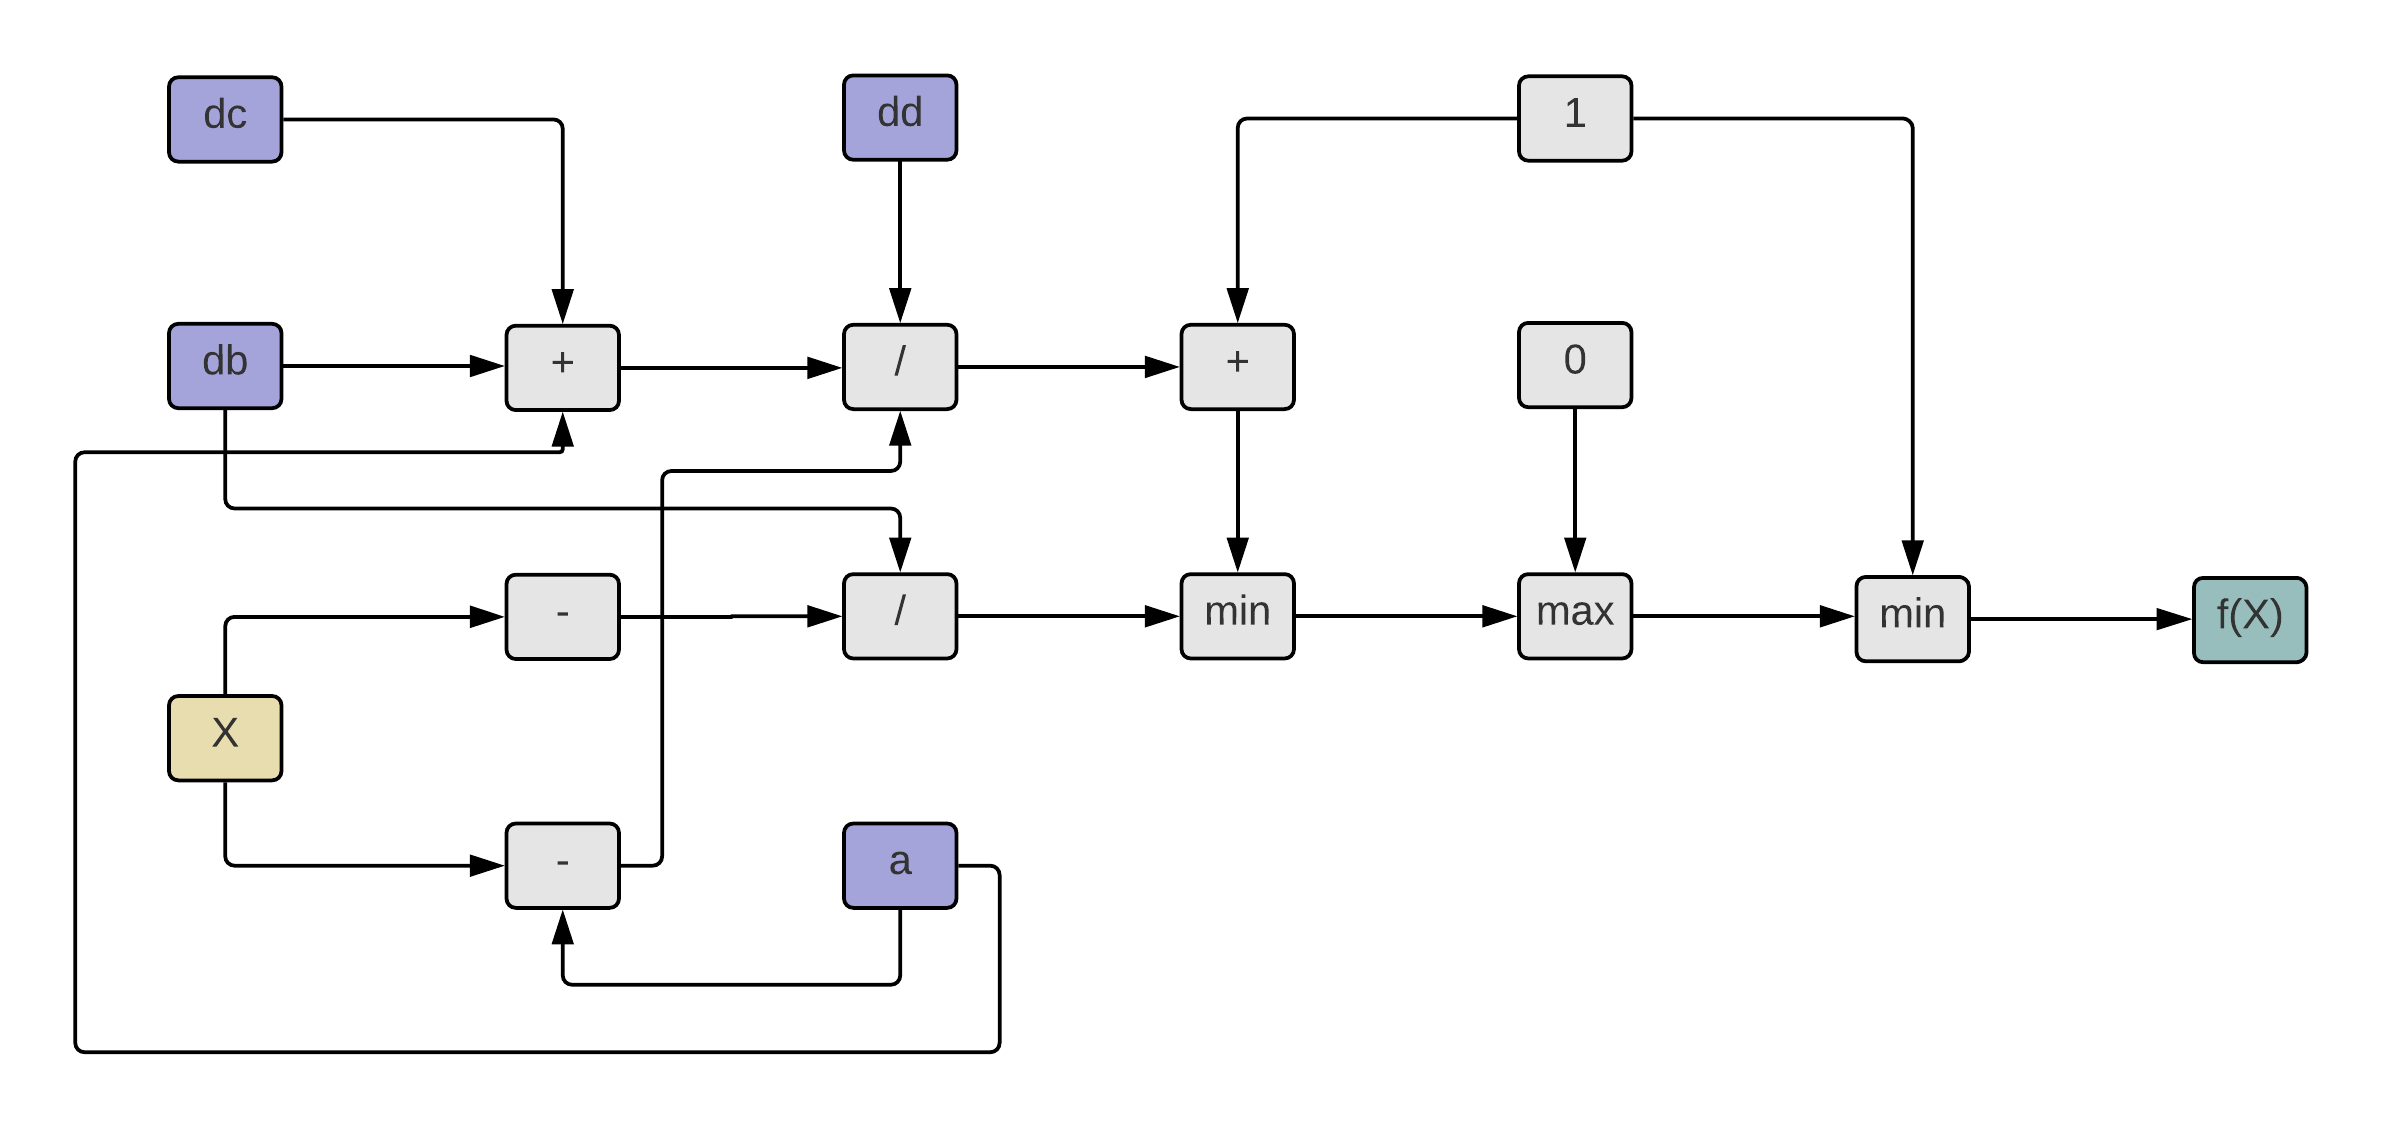
\includegraphics{trap-graph}
	\caption[Grafo computacional de la función de pertenencia para el trapecio]{Ilustración del grafo computacional para la función de pertenencia trapezoidal. La fórmula que describe es $\mu(x) = \min(\max(\min(\mu_{L_{asc}}, \mu_{L_{desc}}), 0), 1)$, esto es, una línea ascendente y otra descendente, estando ambas acotadas en el intervalo $[0, 1] \in \mathbb{R}$.}
	\label{fig:trap-graph}
\end{figure}

Sabiendo los grafos computacionales de cada una de las funciones de pertenencia, podemos definir el grafo asociado a la partición borrosa de una variable lingüística. Suponiendo que la variable $V_i$ está dividida en $N_{V_i}$ conjuntos borrosos\index{conjunto borroso}, la partición estará compuesta de:

\begin{itemize}
	\item Un primer conjunto definido como una pendiente descendente.
	\item $N_{V_i} - 2$ conjuntos definidos como trapezoides.
	\item Un último conjunto definido como una pendiente ascendente.
\end{itemize}

Este grafo tiene que definir una serie de variables para que nuestro algoritmo de entrenamiento las ajuste correctamente. Estas variables están directamente relacionadas con los parámetros de las funciones de pertenencia descritas anteriormente. Hemos decidido por tanto establecer estas variables como los espacios existentes entre los puntos característicos de las funciones.

Al estar definidas de esta manera, logramos (i) que la suma de todas las pertenencias en cada punto del eje $X$ sea $1$ y (ii) que cada pequeña variación del gradiente de una de las variables tiene el potencial de provocar una variación en el resto de variables.

Por último, un \acrlongsp{fcs}\index{sistema de control borroso} define un número de variables de entrada. Nuestro grafo de fuzzificación estará definido de tal manera que para una matriz de entrada $m \times l$, siendo $m$ cada tupla de valores a inferir y $l$ cada una de las variables lingüísticas, generará una matriz de la forma $m \times \sum_{i=1}^l \left\vert{l_i}\right\vert$, siendo $\left\vert{S}\right\vert$ el número de conjuntos borrosos\index{conjunto borroso} que contiene la variable linguística $l_i$ (Figura~\ref{fig:fuzzification-graph})

\begin{figure}
	\centering
	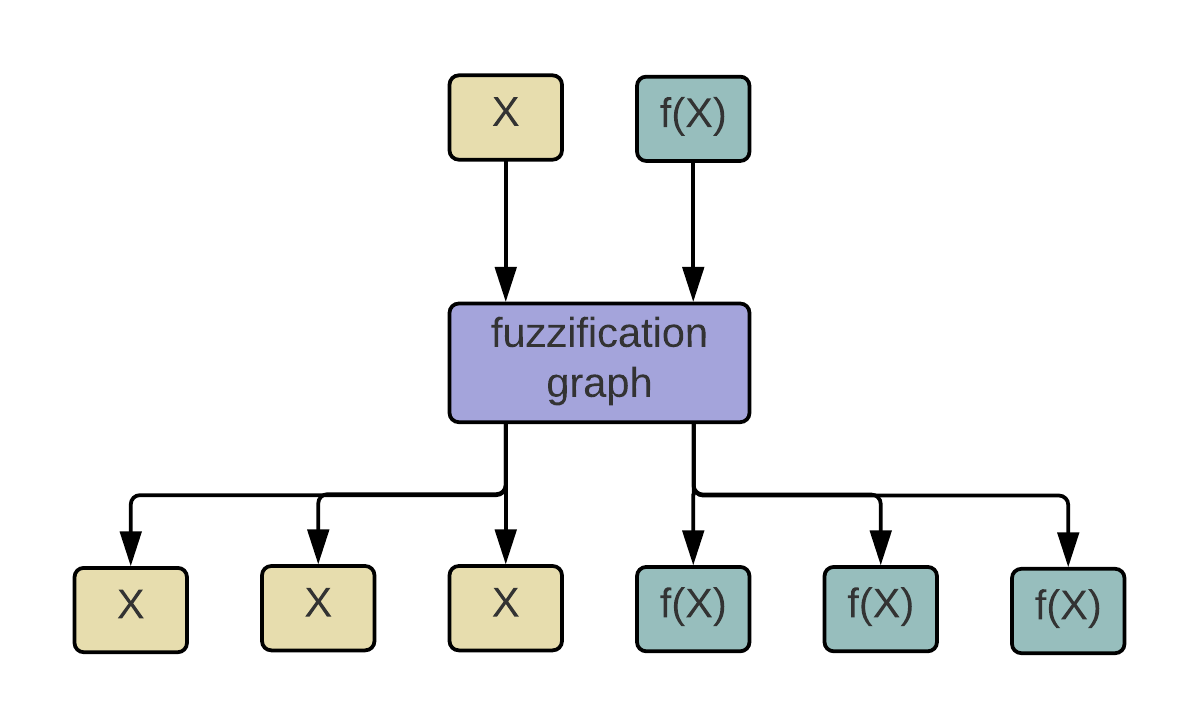
\includegraphics{fuzzification-graph}
	\caption[Ejemplo de operación de fuzzificación como grafo computacional]{Siendo el número de conjuntos borrosos de las variables lingüísticas $X_1$ e $X_2$ $3$, el grafo de fuzzificación transformará los dos valores de entrada $x \in X_1$ e $y \in X_2$ en seis valores, los corerspondientes a los valores de pertenencia de $x$ e $y$ a cada uno de los conjuntos borrosos de $X_1$ y $X_2$ respectivamente}
	\label{fig:fuzzification-graph}
\end{figure}

\paragraph{Bloque de inferencia}

Este bloque tomará una matriz bidimensional de rango $(m, \sum_{i=1}^n N_i)$, es decir, la matriz de salida del bloque de fuzzificación, y generará una matriz bidimensional de rango $(m, N_O)$ que contendrá los valores borrosos de salida (uno por cada conjunto borroso\index{conjunto borroso} de salida). Para ello, hará uso de un bloque de reglas en las que basará su inferencia.

Este bloque de reglas es el que se tratará de ajustar. La representación será la de una matriz $(v_i + 1)$-dimensional, siendo $v_i = \sum_{i=1}^l \left\vert{l_i}\right\vert$ el número total de entradas borrosas que llegan al bloque. La dimensión adicional se corresponde a la variable lingüística de salida.

Dicho de otro modo, cada posible conjunto borroso\index{conjunto borroso} de salida (cada valor dentro del eje correspondiente a la salida) se corresponderá con una matriz $v_i$-dimensional resultado del producto cartesiano de las cariables de entradas. Esto es, cada una de las posibles combinaciones de reglas, a la que podemos asociar un valor. En la Figura~\ref{fig:inference-graph} se muestra un ejemplo con las variables obtenidas en el ejemplo de la Figura~\ref{fig:fuzzification-graph} tras aplicarles la $t$-norma.

\begin{figure}
	\centering
	\begin{equation*}
	\left(\begin{array}{c}
	\mu_1^A \\
	\mu_2^A \\
	\mu_3^A \\
	\end{array}\right)
	\quad \times \quad
	\left(\begin{array}{ c}
	\mu_1^B \\
	\mu_2^B \\
	\mu_3^B \\
	\end{array}\right)
	= \quad 
	\left(\begin{array}{c}
	\top(\mu_1^A, \mu_1^B) \\
	\top(\mu_1^A, \mu_2^B) \\
	\top(\mu_1^A, \mu_3^B) \\
	\top(\mu_2^A, \mu_1^B) \\
	\top(\mu_2^A, \mu_2^B) \\
	\top(\mu_2^A, \mu_3^B) \\
	\top(\mu_3^A, \mu_1^B) \\
	\top(\mu_3^A, \mu_2^B) \\
	\top(\mu_3^A, \mu_3^B) \\
	\end{array}\right)
	\end{equation*}
	\caption[Producto cartesiano de variables borrosas de entrada]{El producto cartesiano de las variables borrosas de entrada genera todas las posibles combinaciones entre los conjuntos borrosos de las variables lingüísticas. Aplicándosele la $t$-norma a cada una de estas combinaciones tenemos todas las posibles reglas que se pueden definir en este \acrlongsp{fcs}.}
	\label{fig:inference-graph}
\end{figure}

Al estar definida la $t$-conorma y la acumulación con el mismo operador, una regla de tipo \texttt{OR} es equivalente a dos reglas de tipo \texttt{AND}, ya que la acumulación de sus resultados es equivalente. Por tanto, al aplicar la $t$-norma a estas combinaciones tenemos todas las posibles combinaciones de reglas. Pero hasta aquí no tenemos ningún ajuste.

Si aplicamos el producto de Hadamard a una matriz de pesos con la misma dimensión y acotamos sus valores a $[0, 1] \in \mathbb{N}$, tenemos una manera de ajustar qué reglas son las más relevantes y cuáles no. Esta representación tiene un problema: estos dos valores definen una función escalón donde el error no se propaga al ser su gradiente $0$. Sin embargo, si en lugar de un valor natural, el peso toma un valor real y le aplicamos una operación sigmoidal, el valor se mantendrá entre $(0, 1) \in \mathbb{R}$ con la ventaja de que el gradiente no se estanca, y en un proceso posterior se pueden descartar las reglas cuyos valores superen ciertos rangos establecidos.

A la salida de la inferencia, tras aplicar la acumulación, disponemos de tantos valores borrosos como conjuntos borrosos tiene la salida.

\paragraph{Bloque de defuzzificación}

Este bloque tiene la particularidad de que no posee ninguna variable que ajustar. Se trata simplemente de una operación que toma una matriz bidimensional de rango $(m, N_O)$ con los valores borrosos de salida y devuelve un vector de rango $(m)$ con los valores en el dominio de la variable lingüística de salida.

\subsection{Ejemplo de ajuste de un \acrlongsp{fcs}\index{sistema de control borroso}}

Se realizará el ajuste de un \acrlongsp{fcs}\index{sistema de control borroso} a partir de un conjunto de entrenamiento con unos valores determinados. Éstos se habrán obtenido a su vez de un \acrlongsp{fcs}\index{sistema de control borroso} de ejemplo para comprobar su correcto funcionamiento.

El ejemplo en concreto se trata del problema clásico de la asignación de propinas, donde la propina viene determinada en función de las variables calidad de la comida y calidad del servicio. Las particiones de las variables lingüísticas del controlador (denominadas \textit{food} y \textit{service}) se muestran en la Figura~\ref{fig:real-tip-controller-vars}.

\begin{figure}
	\centering
	\subfloat[Variable \textit{Food}]{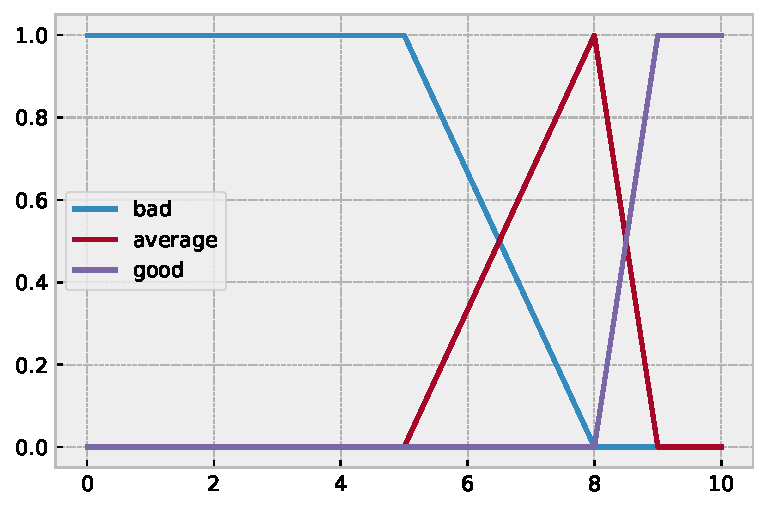
\includegraphics[width=.45\textwidth]{real-tip-controller-var-food}}\qquad
	\subfloat[Variable \textit{Service}]{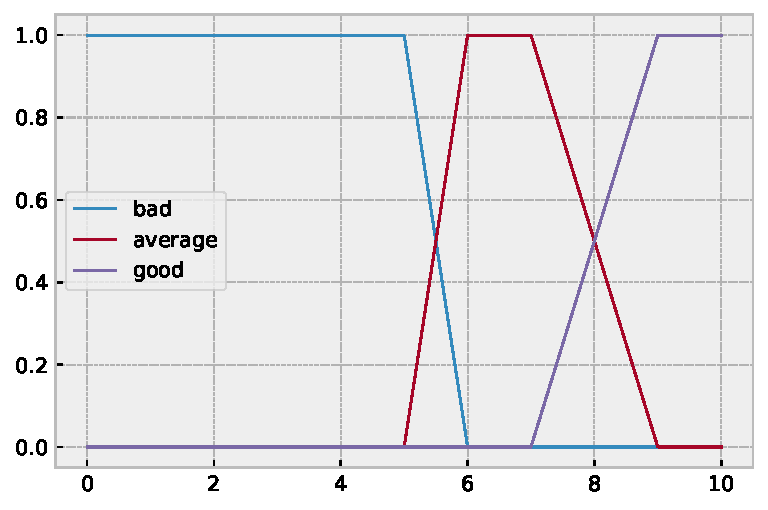
\includegraphics[width=.45\textwidth]{real-tip-controller-var-service}}
	\caption[Particiones borrosas del controlador de ejemplo]{Particiones borrosas del controlador de ejemplo. Estas particiones junto con las reglas definirán la superficie de la función que modela nuestro controlador de ejemplo.}
	\label{fig:real-tip-controller-vars}
\end{figure}

Las reglas que determinan su comportamiento son las siguientes:

\begin{align}
\text{service IS good}                              &\rightarrow \text{tip IS high}\nonumber\\
\text{food IS good}                                 &\rightarrow \text{tip IS high}\nonumber\\
\text{service IS good} \land \text{food IS average} &\rightarrow \text{tip IS low}\nonumber\\
\text{service IS average} \land \text{food IS good} &\rightarrow \text{tip IS high}\nonumber\\
\text{service IS bad}                               &\rightarrow \text{tip IS low}\nonumber\\
\text{food IS bad}                                  &\rightarrow \text{tip IS low}
\end{align}

El controlador es una función con dos variables que describen la superficie mostrada en la Figura~\ref{fig:real-tip-controller-surface}.

\begin{figure}
	\centering
	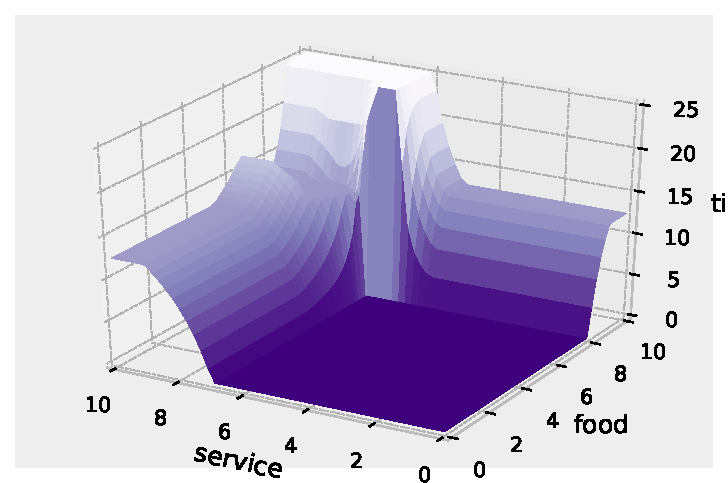
\includegraphics[width=.7\textwidth]{real-tip-controller-surface}
	\caption[Superficie de la función que modela el \acrlongsp{fcs} de ejemplo]{Las reglas y las particiones definen esta función. De ella obtendremos un conjunto de puntos aleatorio para comprobar si nuestra representación de \acrlongsp{fcs} como grafo computacional es capaz de ajustarse a ésta con la técnica del descenso del gradiente.}
	\label{fig:real-tip-controller-surface}
\end{figure}

Recogeremos una muestra aleatoria uniforme de $1500$ puntos de entre los $62500$ que conforman la representación de la superficie del controlador de ejemplo. Posteriormente se creará un controlador borroso y se entrenará aplicando el algoritmo de descenso del gradiente ADAM~\cite{kingma2014adam}.

El proceso de entrenamiento consistirá en la ejecución del algoritmo de propagación del error durante $2500$ epochs con una tasa de aprendizaje de $0.01$, la cual se ha considerado suficiente para el ejemplo en cuestión.

Durante el entrenamiento, las superficies evolucionan hacia una representación aproximada de lo que es el controlador original. En la Figura~\ref{fig:adjusted-tip-controller-training} podemos observar cómo evoluciona la superficie que representa el controlador ajustado.

\begin{figure}
	\centering
	\subfloat[Inicio]{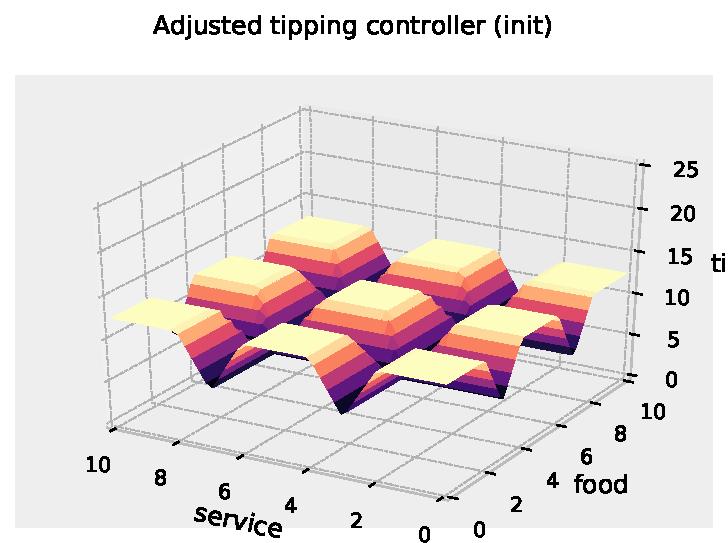
\includegraphics[width=.28\textwidth]{ajusted-tip-controller-at-init-training}}\qquad
	\subfloat[Epoch $250$]{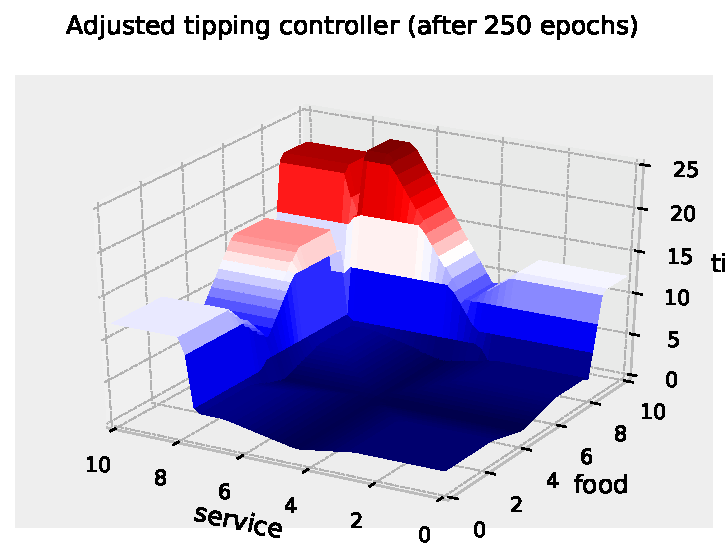
\includegraphics[width=.28\textwidth]{ajusted-tip-controller-at-half-training}}\qquad
	\subfloat[Epoch $500$]{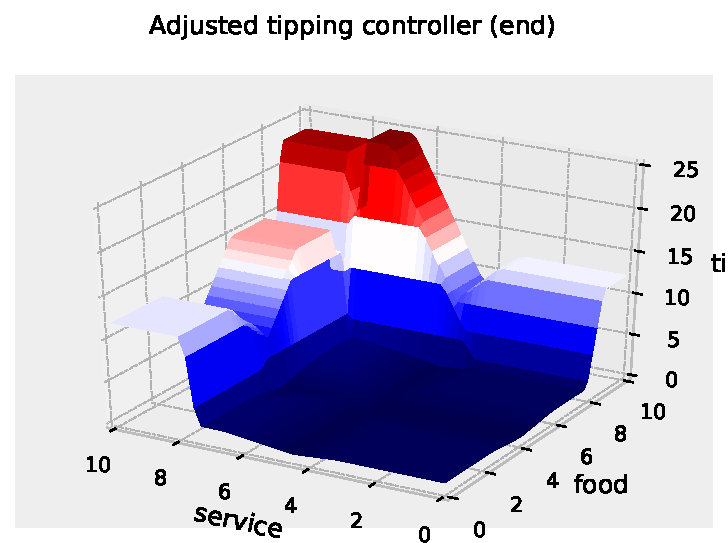
\includegraphics[width=.28\textwidth]{ajusted-tip-controller-at-end-training}}
	\caption[Evolución del \acrlongsp{fcs} de acuerdo al conjunto de datos extraido del ]{Particiones borrosas del \acrlongsp{fcs} de ajustado. Estas figuras muestran la superficie del controlador ajustado (a) al comienzo del proceso de entrenamiento, (b) tras $250$ iteraciones sobre el conjunto de entrenamiento y (c) al final del proceso del entrenamiento.}
	\label{fig:adjusted-tip-controller-training}
\end{figure}

Este proceso demuestra que es posible obtener \acrlongplsp{fcs}\index{sistema de control borroso} ajustados a un patrón de datos con un grado alto de precisión. La ventaja de este método radica en que es posible por tanto explicar mediante reglas el por qué de las predicciones que hace el modelo, a diferencia de otras técnicas como las \acrlongsp{ann}\index{red neuronal artificial}.

\section{Descripción de los datasets}

Del conjunto de datos descrito en la Tabla~\ref{tbl:main-variables} del capítulo~\nameref{ch:methodology} seleccionamos aquellos indicadores de interés: \textit{Distancia a líder}, \textit{Distancia a siguiente TLS}, \textit{Estado de siguiente TLS}, \textit{Velocidad}, \textit{Velocidad a líder} y \textit{Aceleración} (este último como salida a ajustar por el modelo). Estos valores conformarán los conjuntos de entrenamiento y de test tanto para cada uno de los sujetos $S_1$, $S_2$ y $S_3$, como para el conjunto global de éstos $S_A$.

Dado que nuestros modelos se basan en un esquema \textit{\idx{feed-forward}}, existe el inconveniente de que para ellos es imposible mantener una memoria del orden en el que se están sucediendo las entradas. Sin embargo, contamos con las derivadas de la posición respecto al líder (la aceleración y la velocidad al líder) y la velocidad, por lo que consideramos que disponemos de información temporal suficiente para este problema en concreto.

El resultado de la generación de los datasets de entrenamiento y test para todos los sujetos se resume en la Tabla~\ref{tbl:cf-datasets-description}

\section{Modelo basado en \acrlongplsp{fcs}\index{sistema de control borroso}}

\begin{table}[t]
	\centering
	\caption[Descripción de los conjuntos de datos]{Descripción de los conjuntos de datos para el entrenamiento de los modelos. $CF_{S_A}$ se corresponde con el modelo de conductor global, mientras que cada $CF_{S_i}$ es la porción de datos correspondiente al sujeto $S_i$.}
	\label{tbl:cf-datasets-description}
	\begin{tabularx}{\textwidth}{cYYYY}
		\toprule
		& & & \multicolumn{2}{c}{Tamaño} \\
		& Entradas & Salidas & Entrenamiento & Test \\
		\midrule
		\rowcolor{black!20} $CF_{S_1}$ & $7$ & $1$ & $1089$ & $543$ \\
		$CF_{S_2}$ & $7$ & $1$ & $1313$ & $560$ \\
		\rowcolor{black!20} $CF_{S_3}$ & $7$ & $1$ & $2067$ & $668$ \\
		$CF_{S_A}$ & $7$ & $1$ & $4469$ & $1771$ \\
		\bottomrule
	\end{tabularx}
\end{table}

Se han realizado entrenamientos sobre arquitecturas con diferente número de particiones borrosas en las variables. Las arquitecturas que se han considerado más relevantes (tras un proceso de ensayo y error) se describen en la Tabla~\ref{tbl:cf-fcs-architectures}. 

\begin{table*}
	\centering
	\caption[Resumen de las arquitecturas \ac{fcs}\index{sistema de control borroso} para el modelo longitudinal][2em]{Resumen de las arquitecturas seleccionadas. La posición de cada número de la arquitectura indica a qué variable lingüística se refiere (\textit{Distancia al líder}, \textit{Distancia a siguiente TLS}, \textit{TLS en verde}, \textit{TLS en amarillo}, \textit{TLS en rojo}, \textit{Velocidad} y \textit{Velocidad de aproximación al líder} respectivamente). Su valor se corresponde al número de conjuntos borrosos de la partición de cada una de ellas.}
	\label{tbl:cf-fcs-architectures}
	\begin{tabularx}{\linewidth}{cYYYYY}
		\toprule
		\multirow{2}{*}{} & \multirow{2}{*}{Arquitectura} & \multirow{2}{*}{Epochs} & \multicolumn{3}{c}{RMS}      \\ 
		& & & Entrenamiento & Validación & Test \\
		\midrule
		\rowcolor{black!20} $FCS_1$ & $2, 2, 2, 2, 2, 2, 2$ & $10^5$ & $0.059$ & $0.064$ & $0.062$  \\
		$FCS_2$ & $3, 3, 2, 2, 2, 3, 3$ & $10^5$ & $0.073$ & $0.079$ & $0.080$  \\
		\rowcolor{black!20} $FCS_3$ & $4, 3, 2, 2, 2, 3, 3$ & $10^5$ & $0.072$ & $0.078$ & $0.088$  \\
		$FCS_4$ & $5, 5, 2, 2, 2, 5, 5$ & $10^5$ & $0.063$ & $0.068$ & $0.109$  \\
		\bottomrule
	\end{tabularx}
\end{table*}

Todas las arquitecturas mantienen el número de conjuntos borrosos\index{conjunto borroso} asociados a las variables de estado del semáforo (verde, ámbar y rojo) a $2$. La razón es debido a que dicha variable sólo puede tomar dos valores, $0$ o $1$, y en la inicialización de sus respectivas particiones, estas variables ya toman dichos valores con un grado de pertenencia de $1$ en sus dominios.

Cada uno de los controladores se ha entrenado durante $250000$ \textit{epochs}\index{epoch}. En la Figura~\ref{fig:lm-fcs-rmse-all-comparisons} se puede observar la evolución en general y un detalle de la disminución del error durante el entrenamiento de los controladores. El error en test se ofrece a título informativo, y no ha sido usado para determinar las arquitecturas seleccionadas.

\begin{figure}
	\centering
	\subfloat[Entrenamiento y validación]{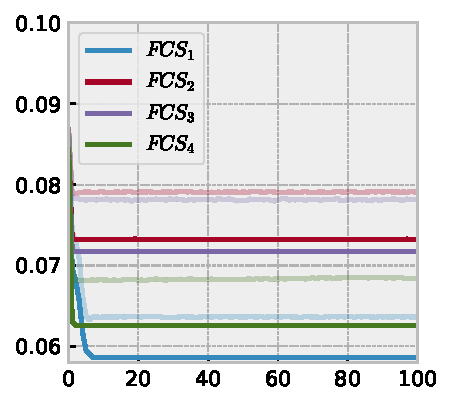
\includegraphics[width=.45\textwidth]{lm-fcs-rmse-all-training-and-validation-detail}}\qquad
	\subfloat[Test]{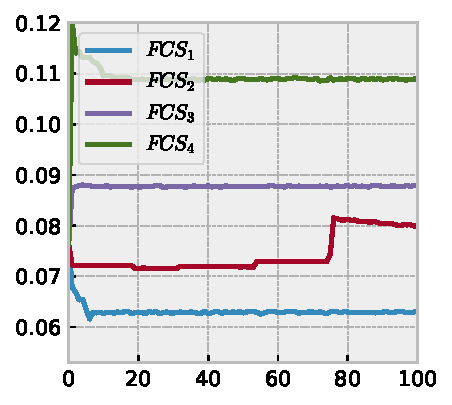
\includegraphics[width=.45\textwidth]{lm-fcs-rmse-all-test-detail}}
	\caption[Evolución del error durante el entrenamiento en las arquitecturas de \acrshort{fcs} para el modelo longitudinal]{Visión en detalle de la evolución del error en los conjuntos de entrenamiento y validación (izquierda) y de test (derecha). Para cada arquitectura, el color más transparente se corresponde al error en el conjunto de validación. El error de test se muestra debido a que nos ofrece puede ofrecer intuición de qué forma aprende la red, pero su evolución no se ha considerado para determinar las arquitecturas.}
	\label{fig:lm-fcs-rmse-all-comparisons}
\end{figure}

En un principio, el proceso de entrenamiento ha sido el habitual, ajustando todas las variables a la vez (particiones borrosas y rreglas). Sin embargo, tras varias pruebas, se ha comprobado que el ajuste de las variables que determinan las particiones borrosas parece suceder más rápido que el ajuste de los pesos asociados a las reglas; por ello, en lugar entrenar a la vez, se ha particionado el entrenamiento en secuencias sucesivas de entrenamiento de reglas y entrenamiento de particiones borrosas.

Concretamente, los $250000$ epochs de entrenamiento han sido divididos en $250$ iteraciones de $800$ epochs ajustando sólo las reglas con una tasa de entrenamiento de $0.01$ seguidos de $200$ epochs ajustando sólo las variables de las particiones borrosas con una tasa de entrenamiento de $0.001$.

En este problema en concreto se ha observado que el entrenamiento realizado de esta manera hace que el \ac{rmse} descienda más rápido en el mismo número de iteraciones. Se puede observar que la arquitectura $FCS_1$ es la que mejor error en test ha alcanzado.

En las pruebas realizadas para el ajuste de controladores se ha observado además que los errores en entrenamiento y en test tienden a ser similares cuando los problemas son representables con un \acrlongsp{fcs}\index{sistema de control borroso}.

Éste será el modelo seleccionado para la comparativa final. Las funciones de pertenencia ajustadas se muestran en la Figura~\ref{fig:adjusted-fuzzy-partitions} contrastadas con las versiones del inicio del entrenamiento, donde $f_i$ se corresponde con la función de pertenencia del conjunto borroso $i$-ésimo de la variable.

\begin{figure}
	\centering
	\subfloat[Distancia a líder (\SI{0}{\meter} a \SI{50}{\meter} norm.)]{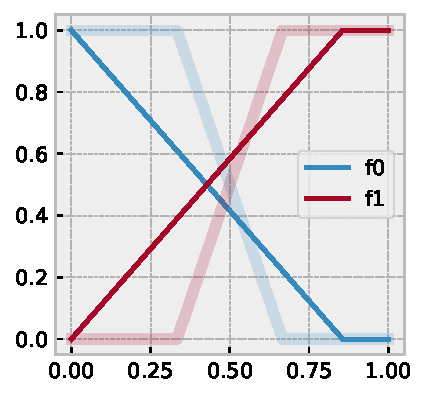
\includegraphics[width=.45\textwidth]{lm-fcs-best-architecture-leader-distance-variable-partition}}\qquad
	\subfloat[Distancia a siguiente semáforo  (\SI{0}{\meter} a \SI{100}{\meter} norm.)]{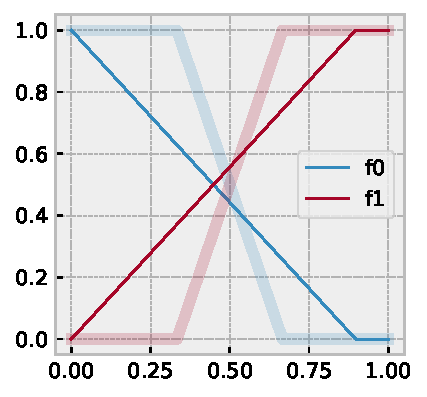
\includegraphics[width=.45\textwidth]{lm-fcs-best-architecture-next-tls-distance-variable-partition}}\qquad
	\subfloat[Velocidad (\SI{0}{\meter\per\second} a \SI{20}{\meter\per\second})]{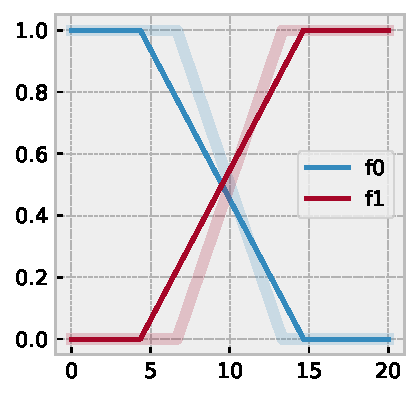
\includegraphics[width=.45\textwidth]{lm-fcs-best-architecture-speed-variable-partition}}\qquad
	\subfloat[Velocidad a líder \SI{-40}{\meter\per\second} a \SI{40}{\meter\per\second})]{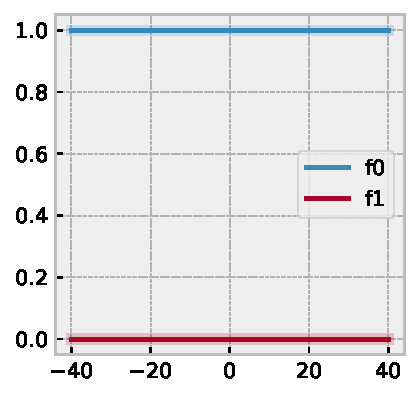
\includegraphics[width=.45\textwidth]{lm-fcs-best-architecture-speed-to-leader-variable-partition}}
	\caption[Particiones borrosas después de la operación de ajuste en el modelo longitudinal basado en \acrshort{fcs}]{Particiones borrosas después de la operación de ajuste en el modelo longitudinal basado en \acrshort{fcs}.}
	\label{fig:adjusted-fuzzy-partitions}
\end{figure}

Las funciones de pertenencia para el estado del semáforo no se incluyen ya que no se vieron modificadas en ningún entrenamiento. Después de todo, estas variables eran binarias, y las particiones borrosas se inicializan de tal manera que dichos valores siempre alcanzan un valor de pertenencia $1$. Las reglas son muy numerosas para ser incluidas en el texto, ya que la mayoría de reglas posibles en el sistema (aproximadamente $60$) tienen un peso asociado de más de $0.5$.

Un detalle que merece la pena destacar es el aprendizaje de la variable lingüística \textit{Velocidad a Líder}. En todos los entrenamientos con las arquitecturas de la Tabla~\ref{tbl:cf-fcs-architectures} el resultado ha sido un único conjunto difuso que cubre todo el dominio de la variable, con todas las reglas de activación teniendo dicho conjunto en cuenta. Esto da indicios de que dicha variable tiene un efecto mínimo o nulo sobre el comportamiento longitudinal, aunque esto contradice a prácticamente todos los modelos de la literatura consultados, por lo que la explicación no puede ser esa. La razón más plausible que podemos encontrar a dicho efecto es que, al tratarse de un entorno urbano, las velocidades que tratamos son muy bajas en comparación con las que se trabaja en este tipo de modelos, y por tanto, la diferencia de velocidades no son un factor determinante en comparación con el resto de variables.

En la Figura~\ref{fig:fcs-test-comparisons} se muestran los perfiles de la aceleración estimada por los controladores frente la aceleración real en cada momento. 

\begin{figure}
	\centering
	\subfloat[Perfil de aceleración]{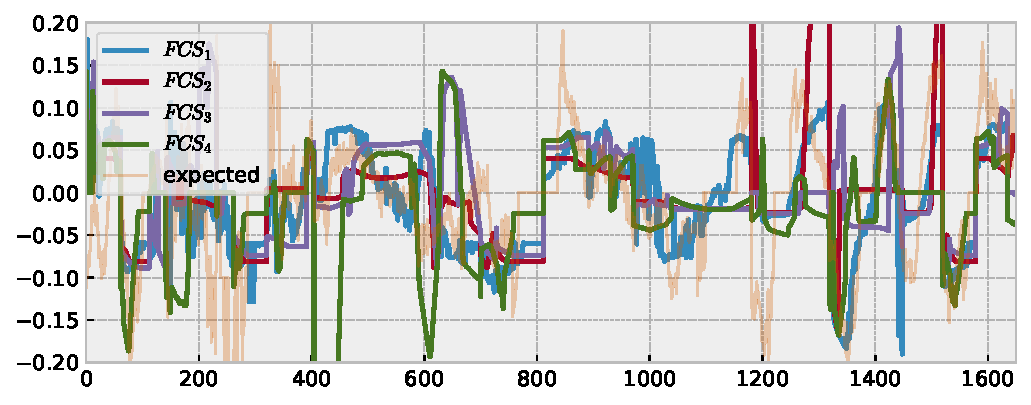
\includegraphics[width=\textwidth]{lm-fcs-outs-all-test-comparison}}\qquad
	\subfloat[Detalle entre frames de $750$ a $1050$]{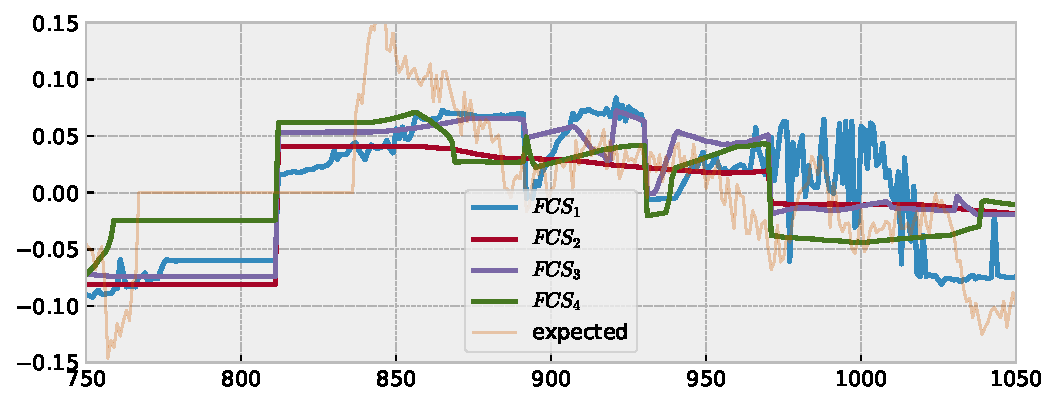
\includegraphics[width=\textwidth]{lm-fcs-outs-all-test-comparison-detail}}
	\caption[Comparación del perfil de aceleración real y el inferido por los modelos entrenados]{Comparación del perfil de aceleración real y el inferido por los modelos entrenados. En la visión general se puede observar el perfile real en color semi-transparente. Debajo, en el perfil, se amplía una pequeña sección del perfil para mostrar los diferentes ajustes de los modelos entrenados y cómo difieren del valor real.}
	\label{fig:fcs-test-comparisons}
\end{figure}

Se puede observar cómo se ajusta el controlador con menor error en test frente al resto. $FCS_1$ presenta picos que aproximan el valor inferido al valor real, mientras que el resto mantiene valores constantes.

\section{Modelo basado en \acrlongplsp{mlp}\index{perceptron multicapa}}

Para determinar el modelo óptimo de \acrlongsp{mlp}\index{perceptron multicapa}, se han realizado entrenamientos sobre arquitecturas con diferente cantidad de neuronas y capas ocultas. Las arquitecturas más ilustrativas de todas las probadas se resumen en la tabla~\ref{tbl:cf-mlp-architectures}.

\begin{table*}
	\centering
	\caption[Resumen de las arquitecturas de \acrlongplsp{mlp} para el modelo longitudinal][2em]{Resumen de las arquitecturas de de \acrlongplsp{mlp} para el modelo longitudinal. La posición de cada número de la topología indica el índice de la capa oculta y su valor el número de nodos (neuronas) que incluye dicha capa. Las arquitecturas seleccionadas en esta tabla son aquellas consideradas relevantes tras un proceso manual de ensayo y error.}
	\label{tbl:cf-mlp-architectures}
	\begin{tabularx}{\linewidth}{cYYYYY}
		\toprule
		\multirow{2}{*}{} & \multirow{2}{*}{Topología} & \multirow{2}{*}{Epochs} & \multicolumn{3}{c}{RMS} \\
		& & & Entrenamiento & Validación & Test \\
		\midrule
		\rowcolor{black!20} $MLP_1$ & $16$        & $10^5$ & $0.057$ & $0.057$ & $0.069$  \\
		$MLP_2$ & $8, 2$      & $10^5$ & $0.061$ & $0.061$ & $0.056$  \\
		\rowcolor{black!20} $MLP_3$ & $16, 8$     & $10^5$ & $0.051$ & $0.051$ & $0.060$  \\
		$MLP_4$ & $16, 16, 8$ & $10^5$ & $0.046$ & $0.046$ & $0.061$  \\
		\bottomrule
	\end{tabularx}
\end{table*}

El modelo de funciones de activación que se ha utilizado es de tipo tangente hiperbólica en todas las neuronas salvo en la última, que se ha utilizado una activación lineal.

En pruebas previas a la selección de estas funciones de activación se han utilizado también funciones de activación de tipo \acrshort{relu}\index{ReLU}, pero las tasas de error tras el entrenamiento eran notablemente más altas por lo que se ha optado al final por el uso de activación basada en tangente hiperbólica. Los pesos de la red han sido inicializados con una muestra aleatoria uniforme de valores reales en el intervalo $(-0.25, 0.25)$.

La Figura~\ref{fig:lm-mlp-rmse-all-comparisons} muestra la evolución del \gls{rmse} durante el proceso de entrenamiento. También se ilustra el error de test, aunque éste no se ha utilizado para decidir las arquitecturas.

\begin{figure}
	\centering
	\subfloat[Entrenamiento y validación]{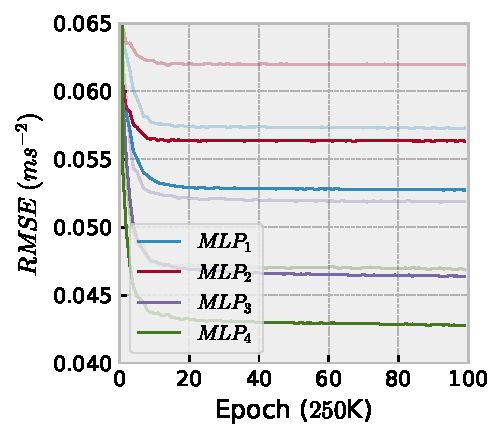
\includegraphics[width=.45\textwidth]{lm-mlp-rmse-all-training-and-validation-detail}}\qquad
	\subfloat[Test]{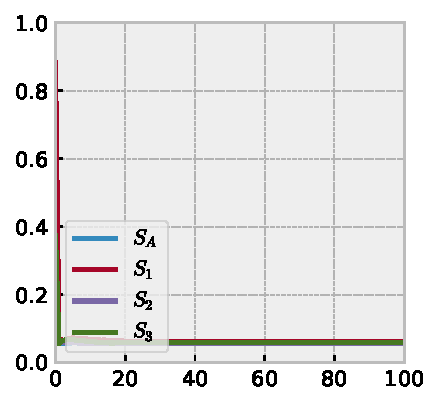
\includegraphics[width=.45\textwidth]{lm-mlp-rmse-all-test-detail}}
	\caption[Evolución del error durante el entrenamiento en las arquitecturas de \acrshort{mlp} para el modelo longitudinal]{Visión en detalle de la evolución del error en los conjuntos de entrenamiento y validación (izquierda) y de test (derecha). Para cada arquitectura, el color más transparente se corresponde al error en el conjunto de validación. El error de test se muestra debido a que nos ofrece puede ofrecer intuición de qué forma aprende la red, pero su evolución no se ha considerado para determinar las arquitecturas.}
	\label{fig:lm-mlp-rmse-all-comparisons}
\end{figure}

Estos errores se encuentran entre los \SI{0.05}{\metre\per\square\second} y los \SI{0.07}{\metre\per\square\second}, lo cual consideramos que es una aproximación aceptable. Una particularidad del problema ha sido la inestabilidad de los entrenamientos, esto es, la alta sensibilidad a los valores de inicialización de los parámetros. La intuición tras observar cómo evolucionan los entrenamientos es que la función de error sufre de muchos mínimos locales o mesetas.

Una visión de detalle del ajuste de estas arquitecturas al conjunto de test se observa en la Figura~\ref{fig:cf-mlp-test-comparisons}, con el perfil de aceleración del conjunto de test y los perfiles de aceleración de las redes entrenadas.

\begin{figure}
	\centering
	\subfloat[Perfil completo]{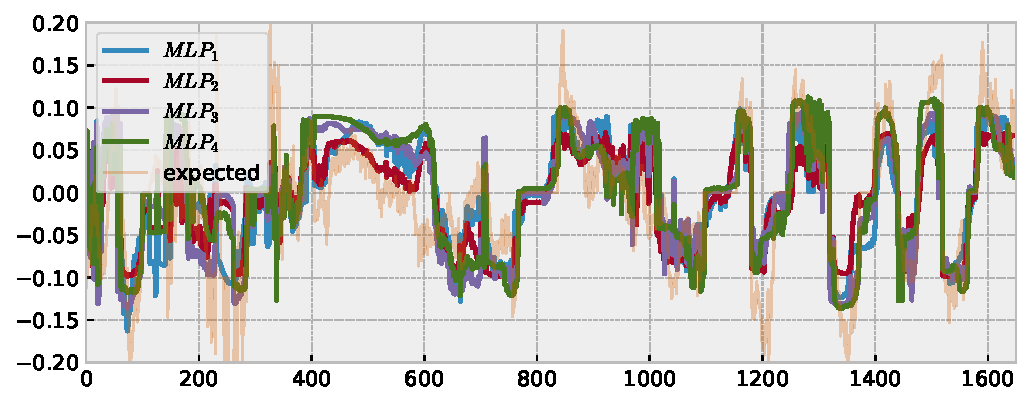
\includegraphics[width=\textwidth]{lm-mlp-outs-all-test-comparison}}\qquad
	\subfloat[Detalle entre frames de $750$ a $1050$]{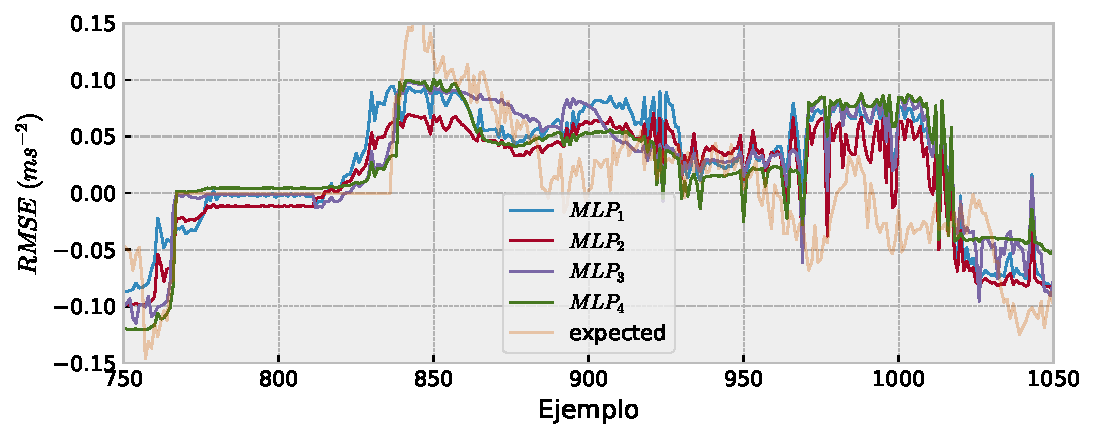
\includegraphics[width=\textwidth]{lm-mlp-outs-all-test-comparison-detail}}
	\caption[Comparación del perfil de aceleración real y el inferido por los modelos entrenados]{Comparación del perfil de aceleración real y el inferido por los modelos entrenados. En la visión general se puede observar el perfil real en semi-transparente. En el detalle, se amplía una pequeña sección del perfil para mostrar los diferentes ajustes de los modelos entrenados y cómo difieren del valor real.}
	\label{fig:cf-mlp-test-comparisons}
\end{figure}

Al contrastar los errores de test, podemos determinar que la arquitectura que mejor generaliza es la $MLP_2$, hecho que se confirma en el ajuste de los perfiles de aceleración. Por lo tanto, parece razonable elegir el modelo $MLP_2$ como candidato para la representación del modelo longitudinal de los conductores.

\section{Comparación entre modelos}

Las mejores arquitecturas de ambos modelos han sido la $MLP_2$ para los \acrlongplsp{mlp}\index{perceptron multicapa} y $FCS_1$ para los \acrlongplsp{fcs}\index{sistema de control borroso}. Los errores y el perfil de aceleración para ambos modelos se muestran en la Figura~\ref{fig:cf-comparison-between-best-mlp-and-fcs-architecture}.

\begin{figure}
	\centering
	\subfloat[Error en test]{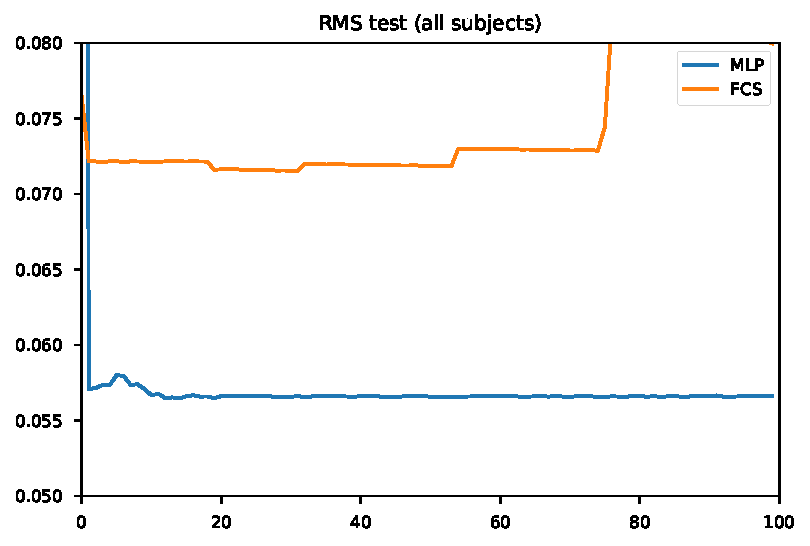
\includegraphics[width=.46\textwidth]{comparison-between-best-mlp-and-fcs-architecture-rms}}\qquad
	\subfloat[Perfil de aceleración]{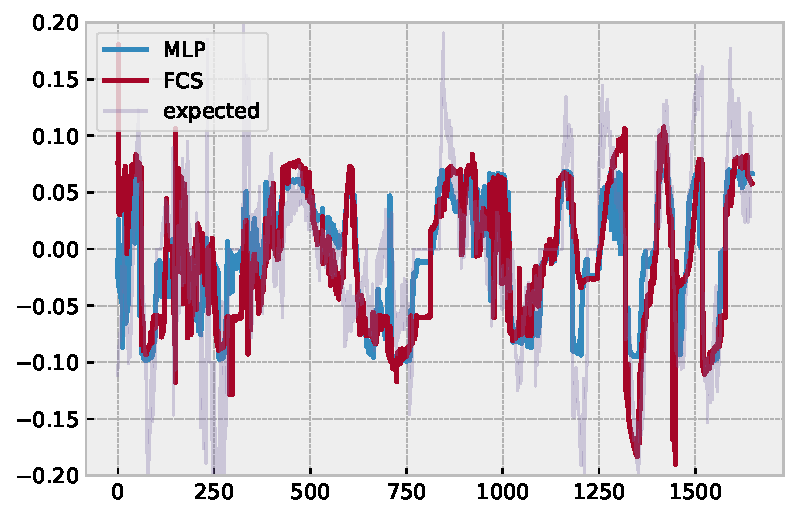
\includegraphics[width=.46\textwidth]{comparison-between-best-mlp-and-fcs-architecture-acceleration-profile}}
	\caption[Comparación entre los dos tipos de modelo longitudinal]{Comparación de la mejor arquitectura de \acrlongplsp{mlp} frente a la mejor arquitectura de \acrlongplsp{fcs}: (a) diferencia entre los errores cuadráticos medios de ambas arquitecturas y (b) perfiles de aceleración en el conjunto de test.}
	\label{fig:cf-comparison-between-best-mlp-and-fcs-architecture}
\end{figure}

Aunque el modelo arroja un error bajo en test, y además tiende a ajustarse al perfil de aceleración, parece que el problema es suficientemente complejo como para no poder representarse como un simple \acrlongsp{fcs}\index{sistema de control borroso}. Además, el error arrojado por el \acrlongsp{mlp}\index{perceptron multicapa} es sustancialmente menor.

Los resultados sugieren por tanto que la arquitectura elegida para el modelo longitudinal será la $MLP_2$.

\section{Modelos longitudinales específicos}

La arquitectura seleccionada ha sido usada para generar los modelos de cada uno de los conductores por separado para comprobar que (i) los errores y precisiones se mantienen en el orden del modelo global, y (ii) capturan las particularidades de cada sujeto de estudio.

En la Figura~\ref{fig:lm-specific-training-validation-and-test-comparison} se muestra la evolución del \gls{rmse}\index{RMSE} en test para cada uno de los sujetos tras entrenar los modelos de arquitectura $MLP_2$ con los datos de los sujetos.

\begin{figure}
	\centering
	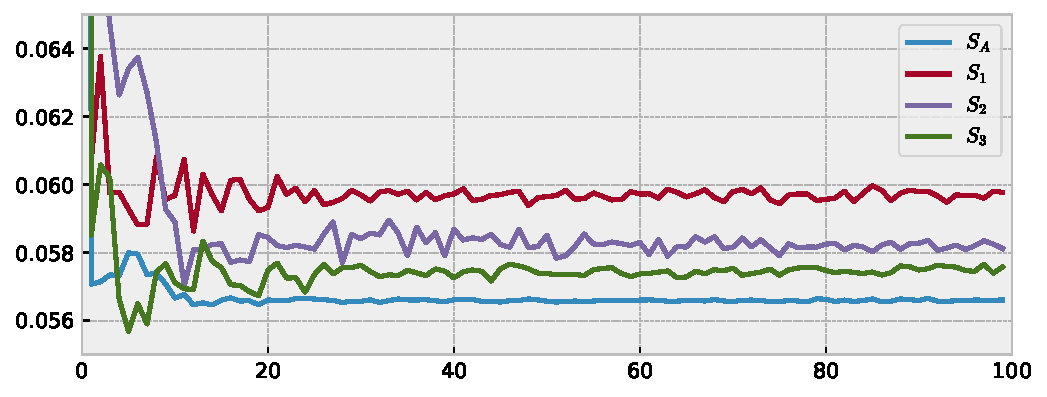
\includegraphics[width=\textwidth]{lm-specific-rmse-all-test-detail}
	\caption[Comparativa de la evolución del \gls{rmse} en test para los sujetos de la arquitectura seleccionada para el modelo longitudinal]{Comparativa de la evolución del error de test entre los sujetos de la arquitectura seleccionada para el modelo longitudinal. El \gls{rmse} en test en el caso del sujeto $S_2$ es muy alto (mayor que $0.2$) comparado con el error en el resto de sujetos y en el global.}
	\label{fig:lm-specific-training-validation-and-test-comparison}
\end{figure}

Se puede observar que el error en test de los sujetos es ligeramente mayor que el del conjunto global. Esto se puede explicar por la mayor capacidad de generalización de $S_A$ al haber sido entrenado con un conjunto de datos mayor. Los errores se resumen en la Tabla~\ref{tbl:lm-specific-rmse}.

\begin{table}
	\centering
	\caption[Resumen de los valores de \Acrshort{rmse} para los modelos específicos de comportamiento longitudinal]{Resumen de los valores de \Acrshort{rmse} para los modelos específicos de comportamiento longitudinal.}
	\label{tbl:lm-specific-rmse}
	\begin{tabularx}{\linewidth}{cYYYYY}
		\toprule
		\multirow{2}{*}{} & \multicolumn{3}{c}{\ac{rmse}}      \\ 
		& Entrenamiento & Validación & Test \\
		\midrule
		\rowcolor{black!20} $S_A$ & $0.056$ & $0.062$ & $0.057$  \\
		$S_1$ & $0.045$ & $0.039$ & $0.060$  \\
		\rowcolor{black!20} $S_2$ & $0.048$ & $0.047$ & $0.058$  \\
		$S_3$ & $0.055$ & $0.054$ & $0.058$  \\
		\bottomrule
	\end{tabularx}
\end{table}

Los resultados parecen sugerir que los errores específicos se mantienen aproximadamente dentro del mismo rango de error que el modelo global. Para verificar que esta topología es capaz de capturar las diferencias entre conductores, comparamos los perfiles de aceleración de los conductores en la Figura~\ref{fig:lm-subjects-comparison}.

En ella se muestra cada perfil de modelo sobre cada uno de los perfiles reales. Podemos observar que, para cada perfil de aceleración, los más similares son los de sus respectivos modelos. En la Tabla~\ref{tbl:lm-subjects-comparison} se describen los \gls{rmse}\index{RMSE} cruzados para de cada uno de los conductores.

\begin{figure}[t]
	\centering
	\subfloat[Sujeto $S_1$]{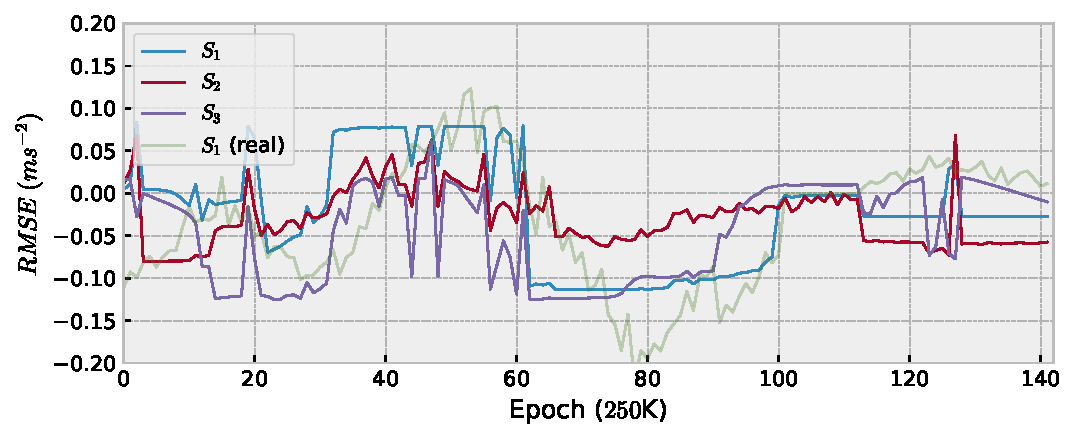
\includegraphics[width=\textwidth]{lm-subjects-comparison-with-edgar-acceleration-profiles}}\qquad
	\subfloat[Sujeto $S_2$]{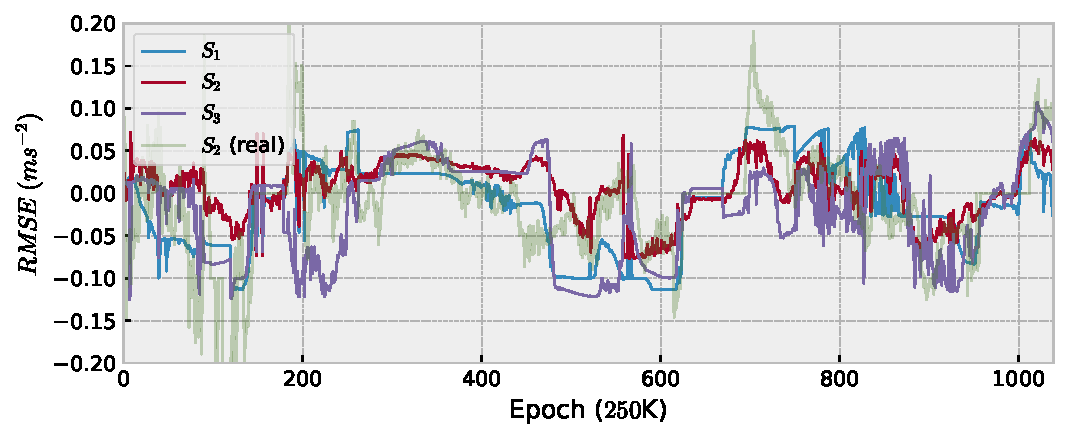
\includegraphics[width=\textwidth]{lm-subjects-comparison-with-jj-acceleration-profiles}}\qquad
	\subfloat[Sujeto $S_3$]{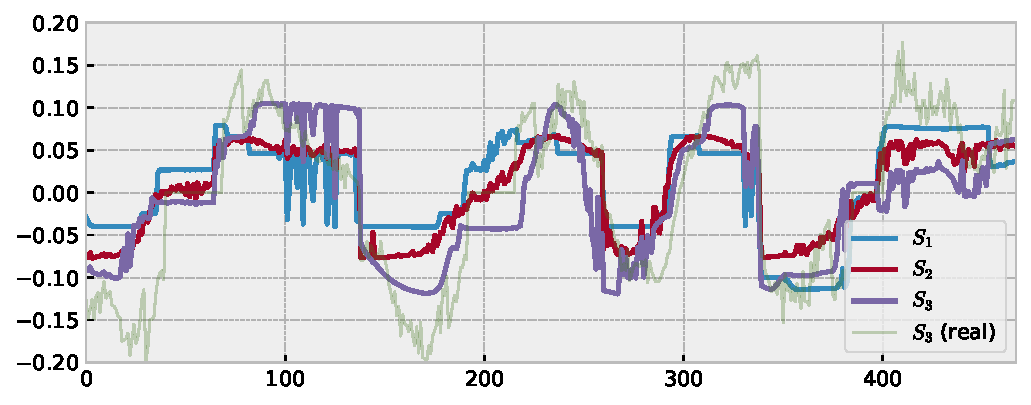
\includegraphics[width=\textwidth]{lm-subjects-comparison-with-miguel-acceleration-profiles}}
	\caption[Diferencia entre los perfiles de aceleración para los diferentes sujetos]{Diferencia entre los perfiles de aceleración para los diferentes sujetos.}
	\label{fig:lm-subjects-comparison}
\end{figure}

\begin{table}
	\centering
	\caption[Comparación de los errores de aceleración en los diferentes modelos longitudinales]{Comparación de los errores de aceleración en los diferentes modelos longitudinales. Las filas se corresponden con los recorridos mientras que las columnas se corresponden con los modelos que se han intentado ajustar a ellas.}
	\label{tbl:lm-subjects-comparison}
	\begin{tabularx}{\linewidth}{YYYY}
		\toprule
		& $S_1$ & $S_2$ & $S_3$ \\
		\midrule
		\rowcolor{black!20} $S_1$ & $0.059$        & $0.074$        & $0.070$ \\
		$S_2$ & $0.064$        & $0.058$        & $0.067$ \\
		\rowcolor{black!20} $S_3$ & $0.065$        & $0.065$        & $0.057$ \\
		\bottomrule
	\end{tabularx}
\end{table}

Se observa que el \gls{rmse}\index{RMSE} es menor cuando el modelo de conductor se aplica sobre los datos del conjunto de test de sus respectivos conductores. Estos modelos basados en la arquitectura $MLP_2$ serán los comportamientos longitudinales de los sujetos en el simulador. Veremos su desempeño en el capítulo \nameref{ch:simulation-implementation}.